%File principale del documento su cui invocare la compilazione, vedi "istruzioni.txt" per più info

%Preambolo: la parte prima del \begin{document}
\documentclass[12pt,a4paper]{article} %formato del documento e grandezza caratteri

%Input del file metadata.tex della cartella locale "res/"
%lista di comandi presenti in template_latex.tex, da qui posso essere modificati secondo le esigenze

\newcommand{\DocTitle}{Verbale interno 2019-11-18} %variabile usata dal file template_latex.tex per settare il titolo del documento
%\newcommand{\DocAuthor}{Progetto "Predire in Grafana"} %variabile usata dal file template_latex.tex per settare l'autore del documento
\newcommand{\DocDate}{18 Novembre 2019} %variabile usata dal file template_latex.tex; Impostata manualmente, altrimenti ad ogni compilazione viene messa la data del giorno di compilazione.
\newcommand{\DocDesc}{Resoconto dell'incontro del gruppo \textit{VRAM Software} tenutosi in data 2019-11-18} %variabile usata dal file template_latex.tex per settare la descrizione del documento
\newcommand{\ver}{27.0.0} %variabile usata dal file template_latex.tex per settare la versione del documento
\newcommand{\app}{Toffoletto Massimo} %variabile usata dal file template_latex.tex per settare l'approvatore del documento
\newcommand{\red}{Dalla Libera Marco} %variabile usata dal file template_latex.tex per settare il redattore del documento
\newcommand{\test}{Schiavon Rebecca} %variabile usata dal file template_latex.tex per settare il verificatore del documento
\newcommand{\stat}{Approvato} %variabile usata dal file template_latex.tex per settare lo stato del documento
\newcommand{\use}{Interno} %variabile usata dal file template_latex.tex per indicare l'uso del documento %Contiene le varibili che descrivono il documento

%Input di file di configurazione presi dalla cartella "Template-LaTeX/config/", uguali per tutti i documenti
%Attenzione bisogna impostare il percorso del file!
% Tutti i pacchetti usati, da inserire nel preambolo prima delle configurazioni

\usepackage[T1]{fontenc} %Permette la sillabazione su qualsiasi testo contenente caratteri
\usepackage[utf8]{inputenc} %Serve per usare la codifica utf-8
\usepackage[english,italian]{babel} %Imposta italiano lingua principale, inglese secondaria. Es. serve per far apparire "indice" al posto di "contents"

\usepackage{graphicx} %Serve per includere le immagini

\usepackage[hypertexnames=false]{hyperref} %Gestisce i riferimenti/link. Es. Serve per rendere clickabili le sezioni dell'indice

\usepackage{float} %Serve per migliore la definizione di oggetti fluttuanti come figure e tabelle. Es. poter usare l'opzione [H] nelle figure ovvero tenere fissate le immagini che altrimenti LaTeX si sposta a piacere.

\usepackage{listings} %Serve per poter mettere snippets di codice nel testo

\usepackage{lastpage} %Serve per poter introdurre un'etichetta a cui si può fare riferimento Es. piè di pagina; poter fare " \rfoot{\thepage\ di \pageref{LastPage}} "

\usepackage{fancyhdr} %Per header e piè di pagina personalizzati

%Sono alcuni package che potranno esserci utili in futuro
%\usepackage{charter}
%\usepackage{eurosym}
\usepackage{subcaption}
%\usepackage{wrapfig}
%\usepackage{background}
\usepackage{longtable} % tabella che può continuare per più di una pagina
\usepackage[table]{xcolor} % ho dovuto aggiungere table in modo da poter colorare le row della tabella, dava: undefined control sequences
%\usepackage{colortbl}

\usepackage{dirtree} % usato per creare strutte tree-view in stile filesystem
\usepackage{xspace} % usato per inserire caratteri spazio
\usepackage[official]{eurosym}
\usepackage{pdflscape} %Inclusione pacchetti
% Configurazioni varie, da inserire nel preambolo dopo i pacchetti

\hypersetup{hidelinks} %serve per nascondere riquadri rossi che circondano i link 

\lstset{literate= {à}{{\`a}}1 } %Permette di usare lettere accentate nei listings

\pagestyle{fancy} %Imposto stile pagina
\fancyhf{} %Reset, se lo tolgo LaTex mette impostazioni di default (p.es numerazione pagine di default)


\lhead{
\includegraphics[scale=0.25]{img/logo_header.png}} %Left header che compare in ogni pagina
%\rhead{\leftmark} %Nome della top-level structure (p.es. Section in article o Chapter in book) in ogni pagina
\rhead{\DocTitle\ v. \ver} %Right header

\newcommand{\glo}{$_G$} %Comando per aggiungere il pedice G
\newcommand{\glosp}{$_G$ } %Comando per aggiungere il pedice G con spazio

\newcommand\Tstrut{\rule{0pt}{2.6ex}} % top padding
\newcommand\Bstrut{\rule[-0.9ex]{0pt}{0pt}} % bottom padding
\newcommand{\TBstrut}{\Tstrut\Bstrut} % top & bottom padding

%Setto il colore dei link
%\hypersetup{
%	colorlinks,
%	linkcolor=[HTML]{404040},
%	citecolor={purple!50!black},
%	urlcolor={blue!50!black}
%}

%Tabelle e tabulazione (può tornare utile)
%\setlength{\tablcolsep}{10pt}
%\renewcommand{\arraystretch}{1.4}

%Comando per aggiungere le pagine di ogni sezione
%\newcommand{\newSection}[1]{%
%	\input{res/sections/#1}
%}

% Comandi per aggiungere padding a parole contenute nella tabella; è una specie di strut (un carattere invisibile)
%\newcommand\Tstrut{\rule{0pt}{2.6ex}} % top padding
%\newcommand\Bstrut{\rule[-0.9ex]{0pt}{0pt}} % bottom padding
%\newcommand{\TBstrut}{\Tstrut\Bstrut} % top & bottom padding  %Configurazione pacchetti

\begin{document}
	%Input del file "frontmatter" preso dalla cartella "Template-LaTeX/config/", uguale per tutti i documenti
	%Attenzione bisogna impostare il percorso del file!
	% #### FRONTESPIZIO (frontmatter) ####
\setlength{\headheight}{33pt} %Distanzia l'header
\pagenumbering{gobble} %Toglie il numero di pagina
\begin{titlepage}
	\begin{center}
		
\includegraphics[scale=0.6]{img/logo.png} \\ %Logo
		\vspace{0.4cm} %Aggiunge uno spazio verticale di 0.5 cm
		
		{\LARGE Progetto "Predire in Grafana"} \\ %Nome progetto
		\vspace{0.4cm} %Attenzione a mettere il punto e NON la virgola
		
		{\Huge \textbf{\DocTitle}} \\ %Titolo, prende variabile definita in metadata.tex
		\vspace{0.4cm}
		
		\DocDate \\ %Data, prende variabile definita in metadata.tex
		\vspace{0.4cm}
		
		%Allineamento colonne: l=left r=right c=center, 
		%va specificato per ogni colonna
		%Se si vuole la riga tra colonne mettere "|"
		
		\begin{tabular}{r | l} %Elementi colonne separate da "&", le righe finiscono con "\\"
			Versione             & \ver \\
			Approvazione         & \app \\ 
			Redazione            & \red \\
			Verifica             & \test \\
			Stato                & \stat \\
			Uso                  & \use \\
		    Destinato a          & Zucchetti \\
						         & Prof. Vardanega Tullio\\
						         & Prof. Cardin Riccardo\\
			Email di riferimento & vram.software@gmail.com
		\end{tabular}
		\vfill
		\textbf{Descrizione} \\
		\DocDesc
	\end{center}
\end{titlepage}
\clearpage

% #### Impostazione header, footer  e numerazione pagine ####
\pagenumbering{arabic} %Pagine con i numeri arabi + reset a 1
\renewcommand{\footrulewidth}{0.4pt} %Di default footrulewidth==0 e quindi è invisibile, di default \headrulewith==0.4pt
\rfoot{\thepage\ di \pageref{LastPage}} %Pagina n di m, con numeri Arabi; usa il pacchetto "lastpage", in caso non sia possibile usare tale pacchetto mettere al fondo dell'ultima pagina "\label{LastPage}"

% #### Tabella dei log ####
% \textbf = grassetto; \Large = font più grande
% \rowcolors{quanti colori alternare}{colore numero riga pari}{colore numero riga dispari}: colori alternati per riga
% \rowcolor{color}: cambia colore di una riga
% p{larghezza colonna}: p è un tipo di colonna di testo verticalmente allineata sopra, ci sarebbe anche m che è centrata a metà ma non è precisa per questo utilizzo TBStrut; la sintassi >{\centering} indica che il contenuto della colonna dovrà essere centrato
% \TBstrut fa parte di alcuni comandi che ho inserito in config.tex che permetto di aggiungere un po' di padding al testo
% \\ [2mm] : questra scrittura indica che lo spazio dopo una break line deve essere di 2mm
% 

%\setcounter{secnumdepth}{0}
%\hfill \break
%\textbf{\Large{Diario delle modifiche}} \\


\addtocontents{toc}{\protect\setcounter{tocdepth}{0}} %Inserire questo per escludere una sezione dall'indice.

\section*{Registro delle modifiche} %Asterisco per fare sezione non numerata
\rowcolors{2}{gray!25}{gray!15}
\begin{longtable} {
		>{\centering}p{17mm} 
		>{\centering}p{19.5mm}
		>{\centering}p{24mm} 
		>{\centering}p{24mm} 
		>{}p{32mm}}
	\rowcolor{gray!50}
	\textbf{Versione} & \textbf{Data} & \textbf{Nominativo} & \textbf{Ruolo} & \textbf{Descrizione} \TBstrut \\
	14.7.0 & 2020-04-09 & Stantagiuliana Vittorio, Toffoletto Massimo e Spreafico Alessandro & \textit{Progettista}, \textit{Verificatore} e \textit{Responsabile di progetto} & Stesura, verifica e approvazione documento. \TBstrut \\ [2mm]
\end{longtable}

\addtocontents{toc}{\protect\setcounter{tocdepth}{4}} %Inserire questo per ripristinare il normale inserimento delle sezioni nell'indice. 4 significa fino al paragrah
\clearpage

% #### INDICE (tableofcontents) ####
\tableofcontents %Provoca la stampa dell'indice
\clearpage

\setcounter{secnumdepth}{4} %Permette di andare fino alla profondità del paragraph con la numerazione delle sezioni %Imposta il frontespizio, l'indice, header e footer
	
	%Tutte le sezioni del documento
	\subsection{Installazione di Grafana}
Per installare Grafana\glo, visitare la pagina \url{https://grafana.com/get}. Qui è possibile trovare il download per MacOS, Windows e sistemi operativi basati su Linux/Unix.
\subsubsection{Eseguire il servizio WEB Grafana} Per eseguire il servizio WEB Grafana\glo, aprire la cartella "bin" dell'installazione Grafana\glosp ed a seconda del sistema operativo eseguire:
\begin{itemize}
	\item \textbf{Windows}: doppio click sul file "grafana-server";
	\item \textbf{Linux e Mac}: eseguire in una shell il comando:
		\begin{verbatim}
			./grafana-server web
		\end{verbatim}
\end{itemize}
Collegarsi quindi con un browser all'indirizzo \url{http://localhost:3000/}. Le credenziali richieste al primo avvio sono username "admin" e password "admin".
\begin{center}
%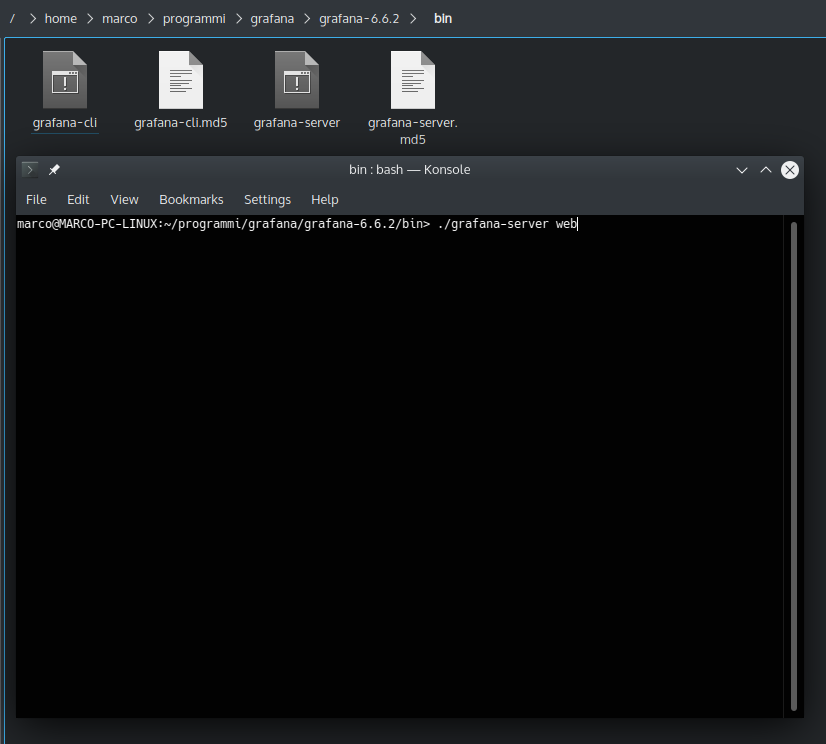
\includegraphics[width=10cm,height=\textheight,keepaspectratio]{img/grafana-server.png}
%\mbox{}\\ [5mm]
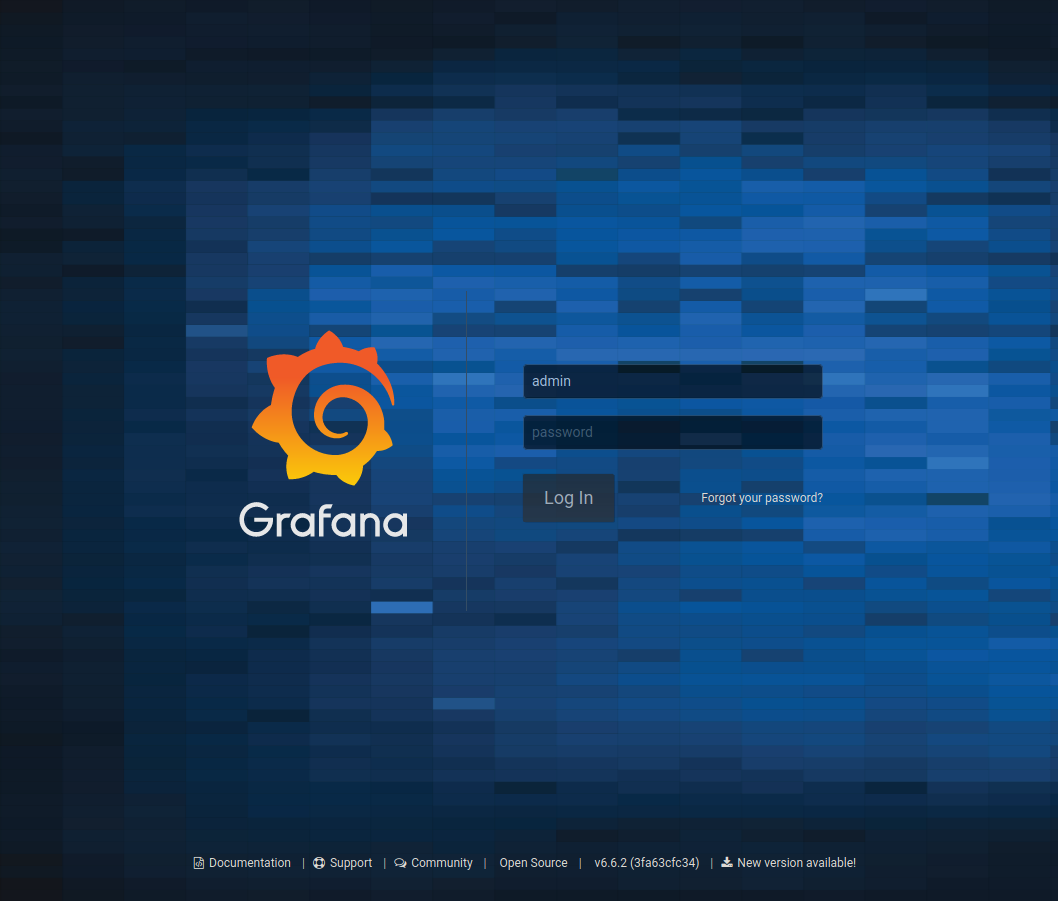
\includegraphics[width=10cm,height=\textheight,keepaspectratio]{img/grafana-login.png}
\end{center}

%\subsection{Installazione plug-in Grafana}
%\subsubsection{Requisiti}
%\begin{itemize}
%	\item \textbf{Grafana\glo};
%	\item \textbf{Node.js}: runtime Javascript che permette di eseguire codice Javascript fuori da un browser. L'installazione di npm (Node Package Manager) non è richiesta dato che viene installato automaticamente durante l'installazione di Node.js;
%	\item \textbf{Git}: sistema di versionamento distribuito.
%\end{itemize}

\subsection{Installazione del plug-in}
\subsubsection{Clonare la repository da GitHub}%\mbox{}\\ [1mm]
Per clonare la repository dell'applicazione, aprire un terminale e usare il comando cd per spostarsi in una cartella a propria scelta ed eseguire il comando:
\begin{verbatim}
	git clone https://github.com/VRAM-Software/grafana_prediction.git
\end{verbatim}
Infine con il comando 
\begin{verbatim}
	cd ./grafana_prediction_plugin
\end{verbatim}
si accede alla cartella che contiene il codice sorgente del plug-in.

\subsubsection{Installare le dipendenze}%\mbox{}\\ [1mm]
Per il corretto funzionamento dell'applicazione è necessario installare tutte le dipendenze elencate precedentemente. Per farlo eseguire il comando:
\begin{verbatim}
	npm install
\end{verbatim}

\subsubsection{Eseguire il plug-in}%\mbox{}\\ [1mm]
Per eseguire l'applicazione è necessario copiare il contenuto del repository "grafana\_prediction\_plugin", ad eccezione delle cartelle "node\_modules" e "coverage", all'interno della cartella "data/plugins" dell'installazione Grafana\glo. Accedendo all'interfaccia web si potrà quindi abilitare il plug-in dall'apposita sezione plug-in delle impostazioni.
\\
\\
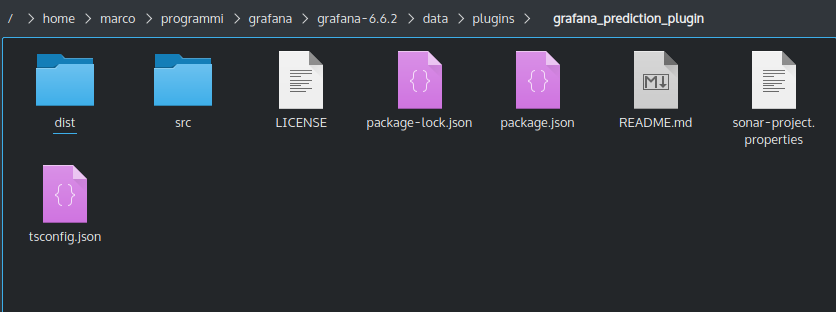
\includegraphics[width=\textwidth,height=\textheight,keepaspectratio]{img/plugin-directory.png}

\subsubsection{Impacchettare il plug-in}%\mbox{}\\ [1mm]
Per generare una release di produzione basta eseguire il comando:
\begin{verbatim}
	npm run build	
\end{verbatim}
e successivamente creare un archivio zip dell'intero repository escludendo le cartelle "node\_modules" e "coverage". Questo plug-in potrà poi esser distribuito e installato da altri utenti. 

	\section{Configurazione dell'ambiente di lavoro}
\subsection{Configurazione ambiente di sviluppo integrato WebStorm}
La configurazione base di WebStorm prevede la corretta configurazione dei path di sistema e l'apertura di un progetto.
\subsubsection{Configurazione dei path di sistema}
Aprire le impostazioni di WebStorm dal suo menù "File" ed utilizzando la barra di ricerca cercare "Node.js and NPM". Verificare quindi che entrambe le voci "Node interpreter" e "Package manager" siano correttamente impostate.
\\
\\
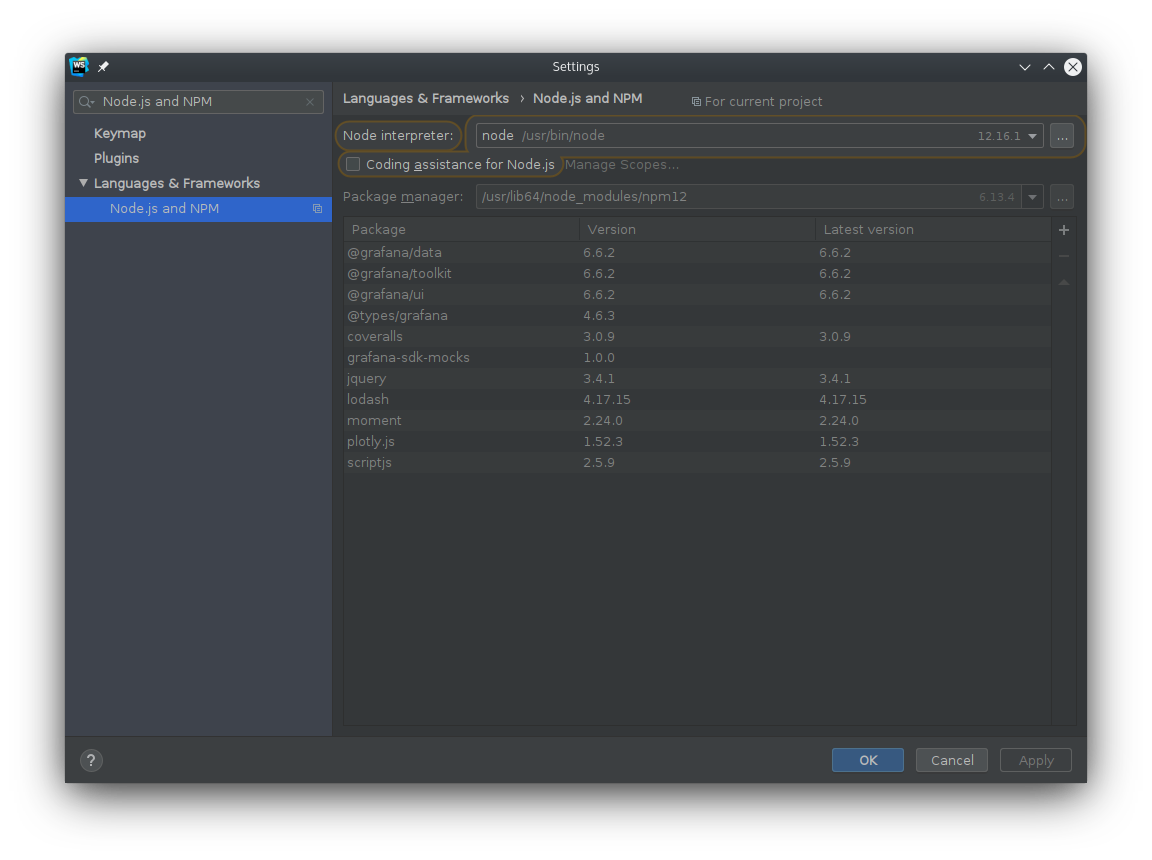
\includegraphics[width=\textwidth,height=\textheight,keepaspectratio]{img/node-npm.png}
\subsubsection{Importazione di un progetto}
Dal menu "File" selezionare la voce "Open" e successivamente la root directory del repository desiderato.

\pagebreak
\subsection{Configurazione plug-in SonarLint per WebStorm}
\subsubsection{Configurazione globale}
Per configurare il plug-in SonarLint, aprire le impostazioni di WebStorm dal suo menù "File". Quindi nella sezione "Tools" selezionare la voce "SonarLint". Nella finestra visualizzare selezionare il "+" per aggiungere una connessione al servizio WEB SonarCloud.
\\
\\
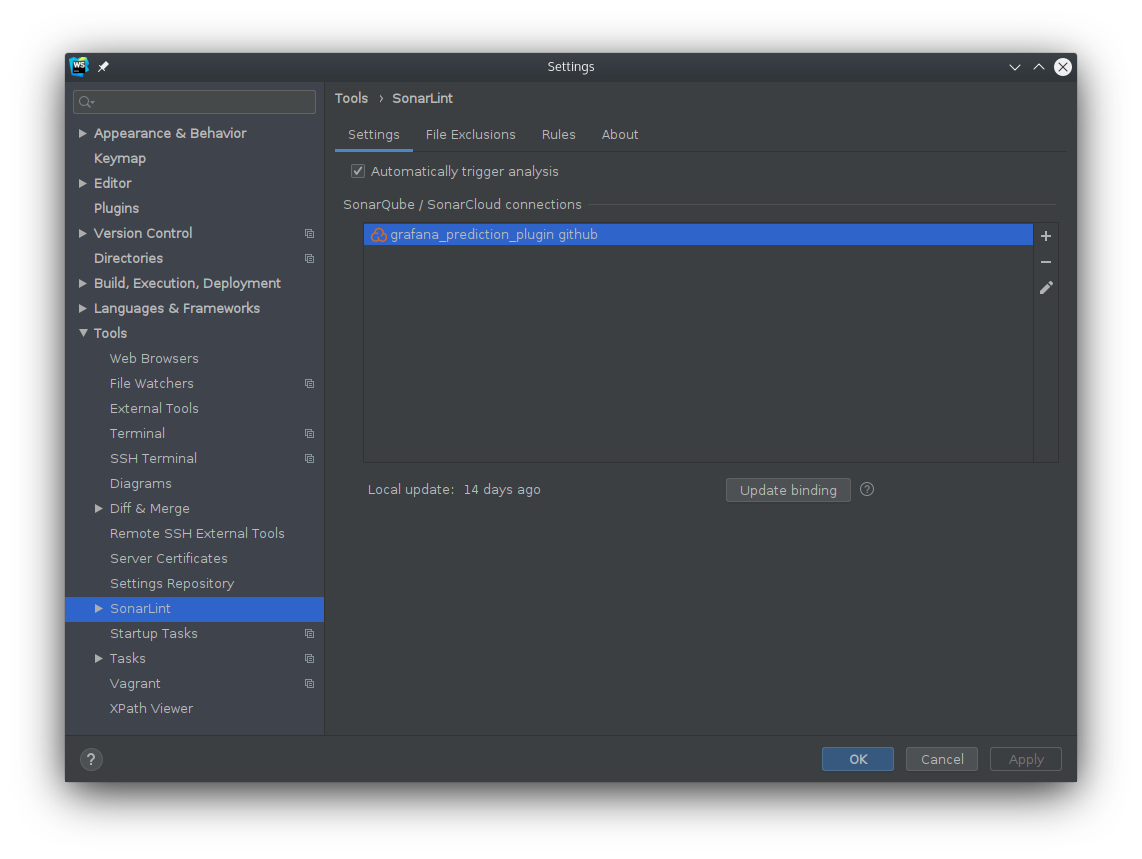
\includegraphics[width=\textwidth,height=\textheight,keepaspectratio]{img/connection.png}
\pagebreak
\\
Dare un nome al collegamento e selezionare SonarCloud, successivamente premere "Next".
\\
\\
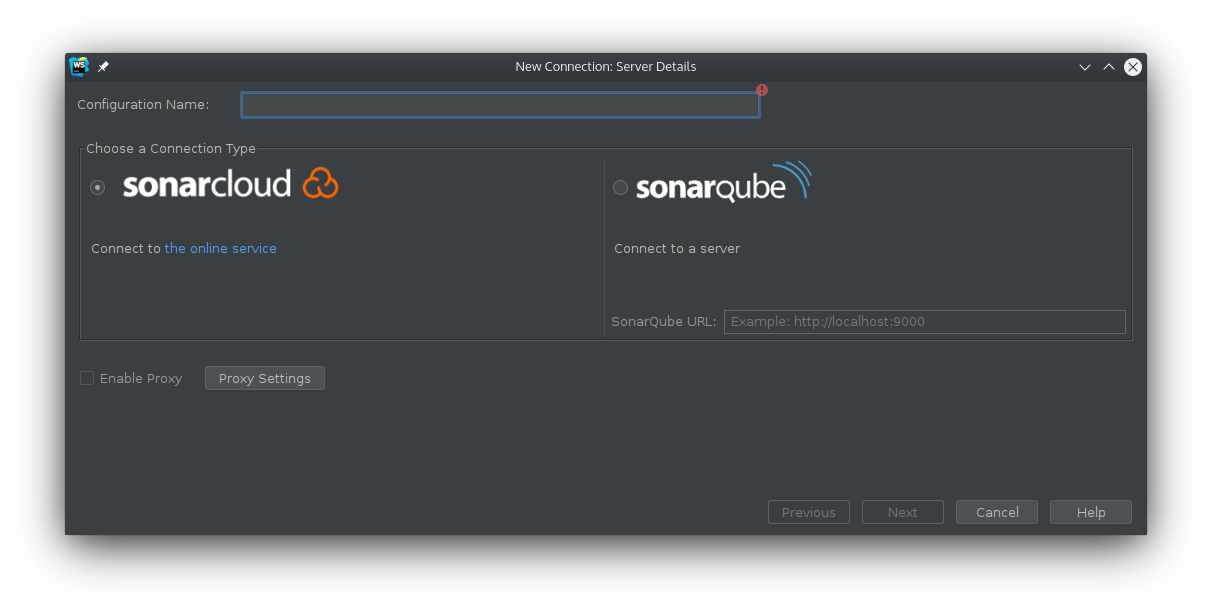
\includegraphics[width=\textwidth,height=\textheight,keepaspectratio]{img/connection-name.png}
\\
Premere su "Create Token".
\\
\\
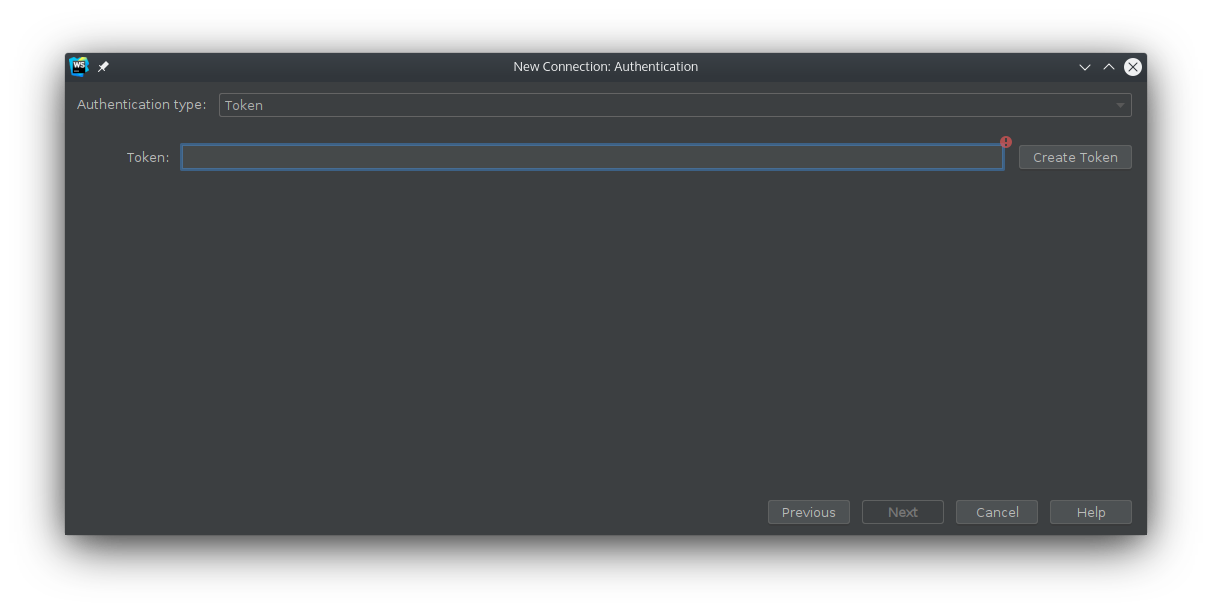
\includegraphics[width=\textwidth,height=\textheight,keepaspectratio]{img/token.png}
\\
Scegliere un nome e creare il token, copiarlo quindi nella finestra WebStorm precedente.
%\\
%\\
%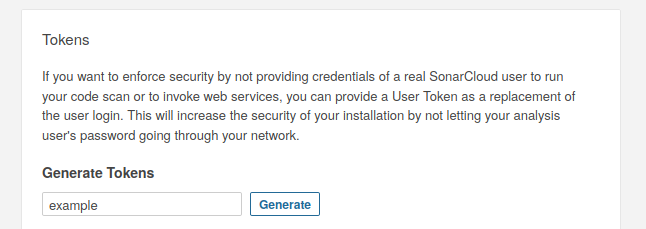
\includegraphics[width=\textwidth,height=\textheight,keepaspectratio]{img/sonarcloud.png}
La connessione viene verificata ed è possibile visualizzarla nell'elenco delle connessioni.
\subsubsection{Configurazione per progetto}
Dopo aver terminato la configurazione globale è possibile configurare i singoli progetti. Per farlo aprire le impostazioni di WebStorm dal suo menù "File", Quindi nella sezione "Tools" espandere la voce "SonarLint" e selezionare "Project Settings".
\\
\\
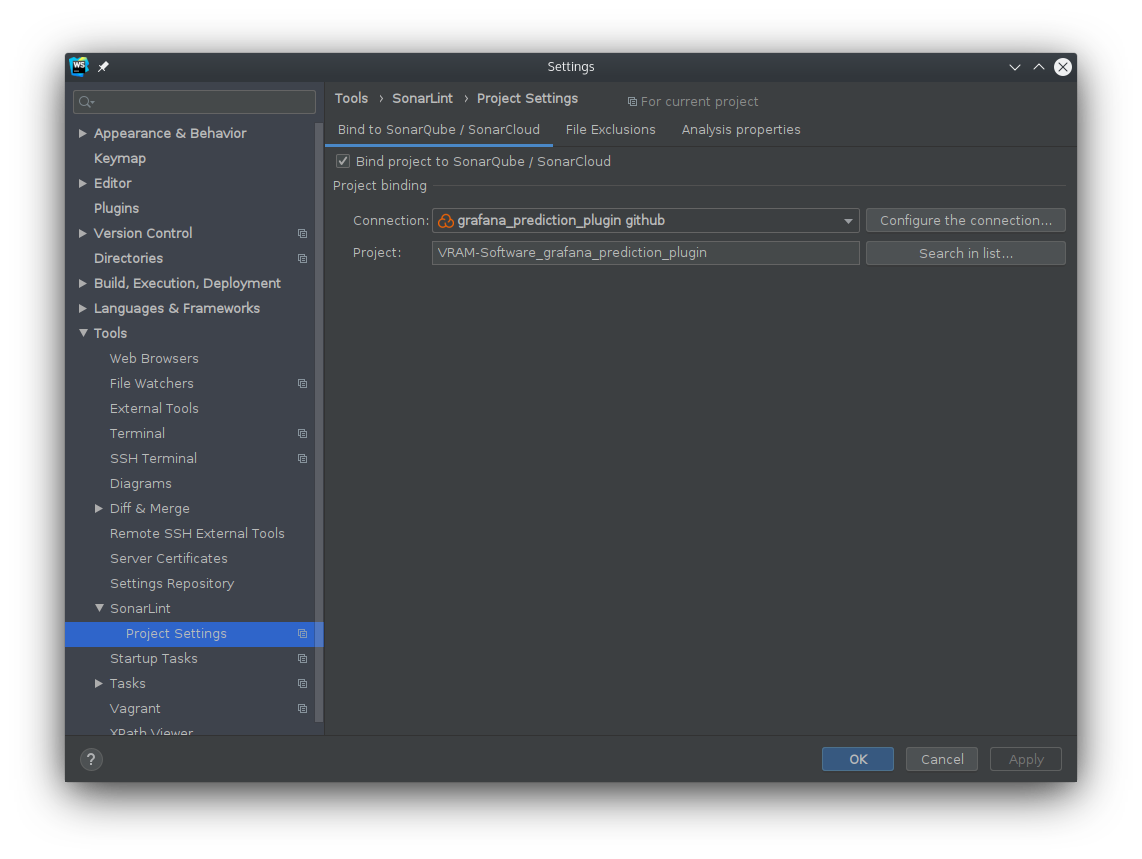
\includegraphics[width=\textwidth,height=\textheight,keepaspectratio]{img/sonarlint-project.png}
Selezionare la connessione a SonarCloud desiderata ed inserire una delle chiavi seguenti, a seconda del progetto che si sta configurando:
\begin{itemize}
	\item \textbf{plug-in Grafana}: VRAM-Software\_grafana\_prediction\_plugin;
	\item \textbf{Applicativo esterno}: VRAM-Software\_prediction\_configuration\_utility.
\end{itemize}

\subsection{Configurazione ambiente plug-in Grafana}
\subsubsection{Contenuto file package.json}
Il file package.json contiene tutte le informazioni e i requisiti necessari della nostra applicazione. Le informazioni importanti sono i seguenti attributi:
\begin{itemize}
	\item dependencies: contiene la seguente lista di pacchetti che sono necessari per il corretto funzionamento dell'applicazione:
		\begin{itemize}
			\item jquery;
			\item lodash;
			\item moment;
			\item plotly.js;
			\item scriptjs.
		\end{itemize}
	\item devDependencies: questo attributo contiene la seguente lista di pacchetti che sono necessari per il corretto funzionamento dell'applicazione durante lo sviluppo:
		\begin{itemize}
			\item @grafana/data;
			\item @grafana/toolkit;
			\item @grafana/ui;
			\item @types/grafana;
			\item grafana-sdk-mocks;
			\item coveralls.
		\end{itemize}
	\item{scripts}: questo attributo contiene una lista di tutti i comandi, utili per uno sviluppatore, che possono essere eseguiti da linea di comando:
		\begin{itemize}
			\item \textbf{build}: il comando seguente genera una cartella chiamata dist che contiene i file di produzione del plug-in Grafana\glo;
			\begin{verbatim}
				npm run build
			\end{verbatim}
			\item \textbf{test}: il comando fa eseguire tutti i test automatici dell'applicazione;
			\begin{verbatim}
				npm test
			\end{verbatim}
			\item \textbf{dev}: il comando genera una release di debug da utilizzare durante lo sviluppo, eseguendo inoltre i linting integrati nella dipendenza npm @grafana/toolkit. Non esegue i test automatici;
			\begin{verbatim}
				npm run dev
			\end{verbatim}
			\item \textbf{ci-test}: il comando, pensato per essere eseguito nell'ambiente di continuous integration, fa eseguire tutti i test automatici dell'applicazione e calcola il code coverage del codice;
			\begin{verbatim}
				npm run ci-test
			\end{verbatim}
			\item \textbf{watch}: il comando esegue il comando "dev" in modalità "watch", ovvero segnalando in automatico gli errori di linting durante la scrittura del codice.
			\begin{verbatim}
				npm run watch
			\end{verbatim}
		\end{itemize}
\end{itemize}

	% ...
	%\input{res/inserire nome sezione n} 
\end{document}